\specialsection{Introduction}{}{black}{white}

\begin{figure}
    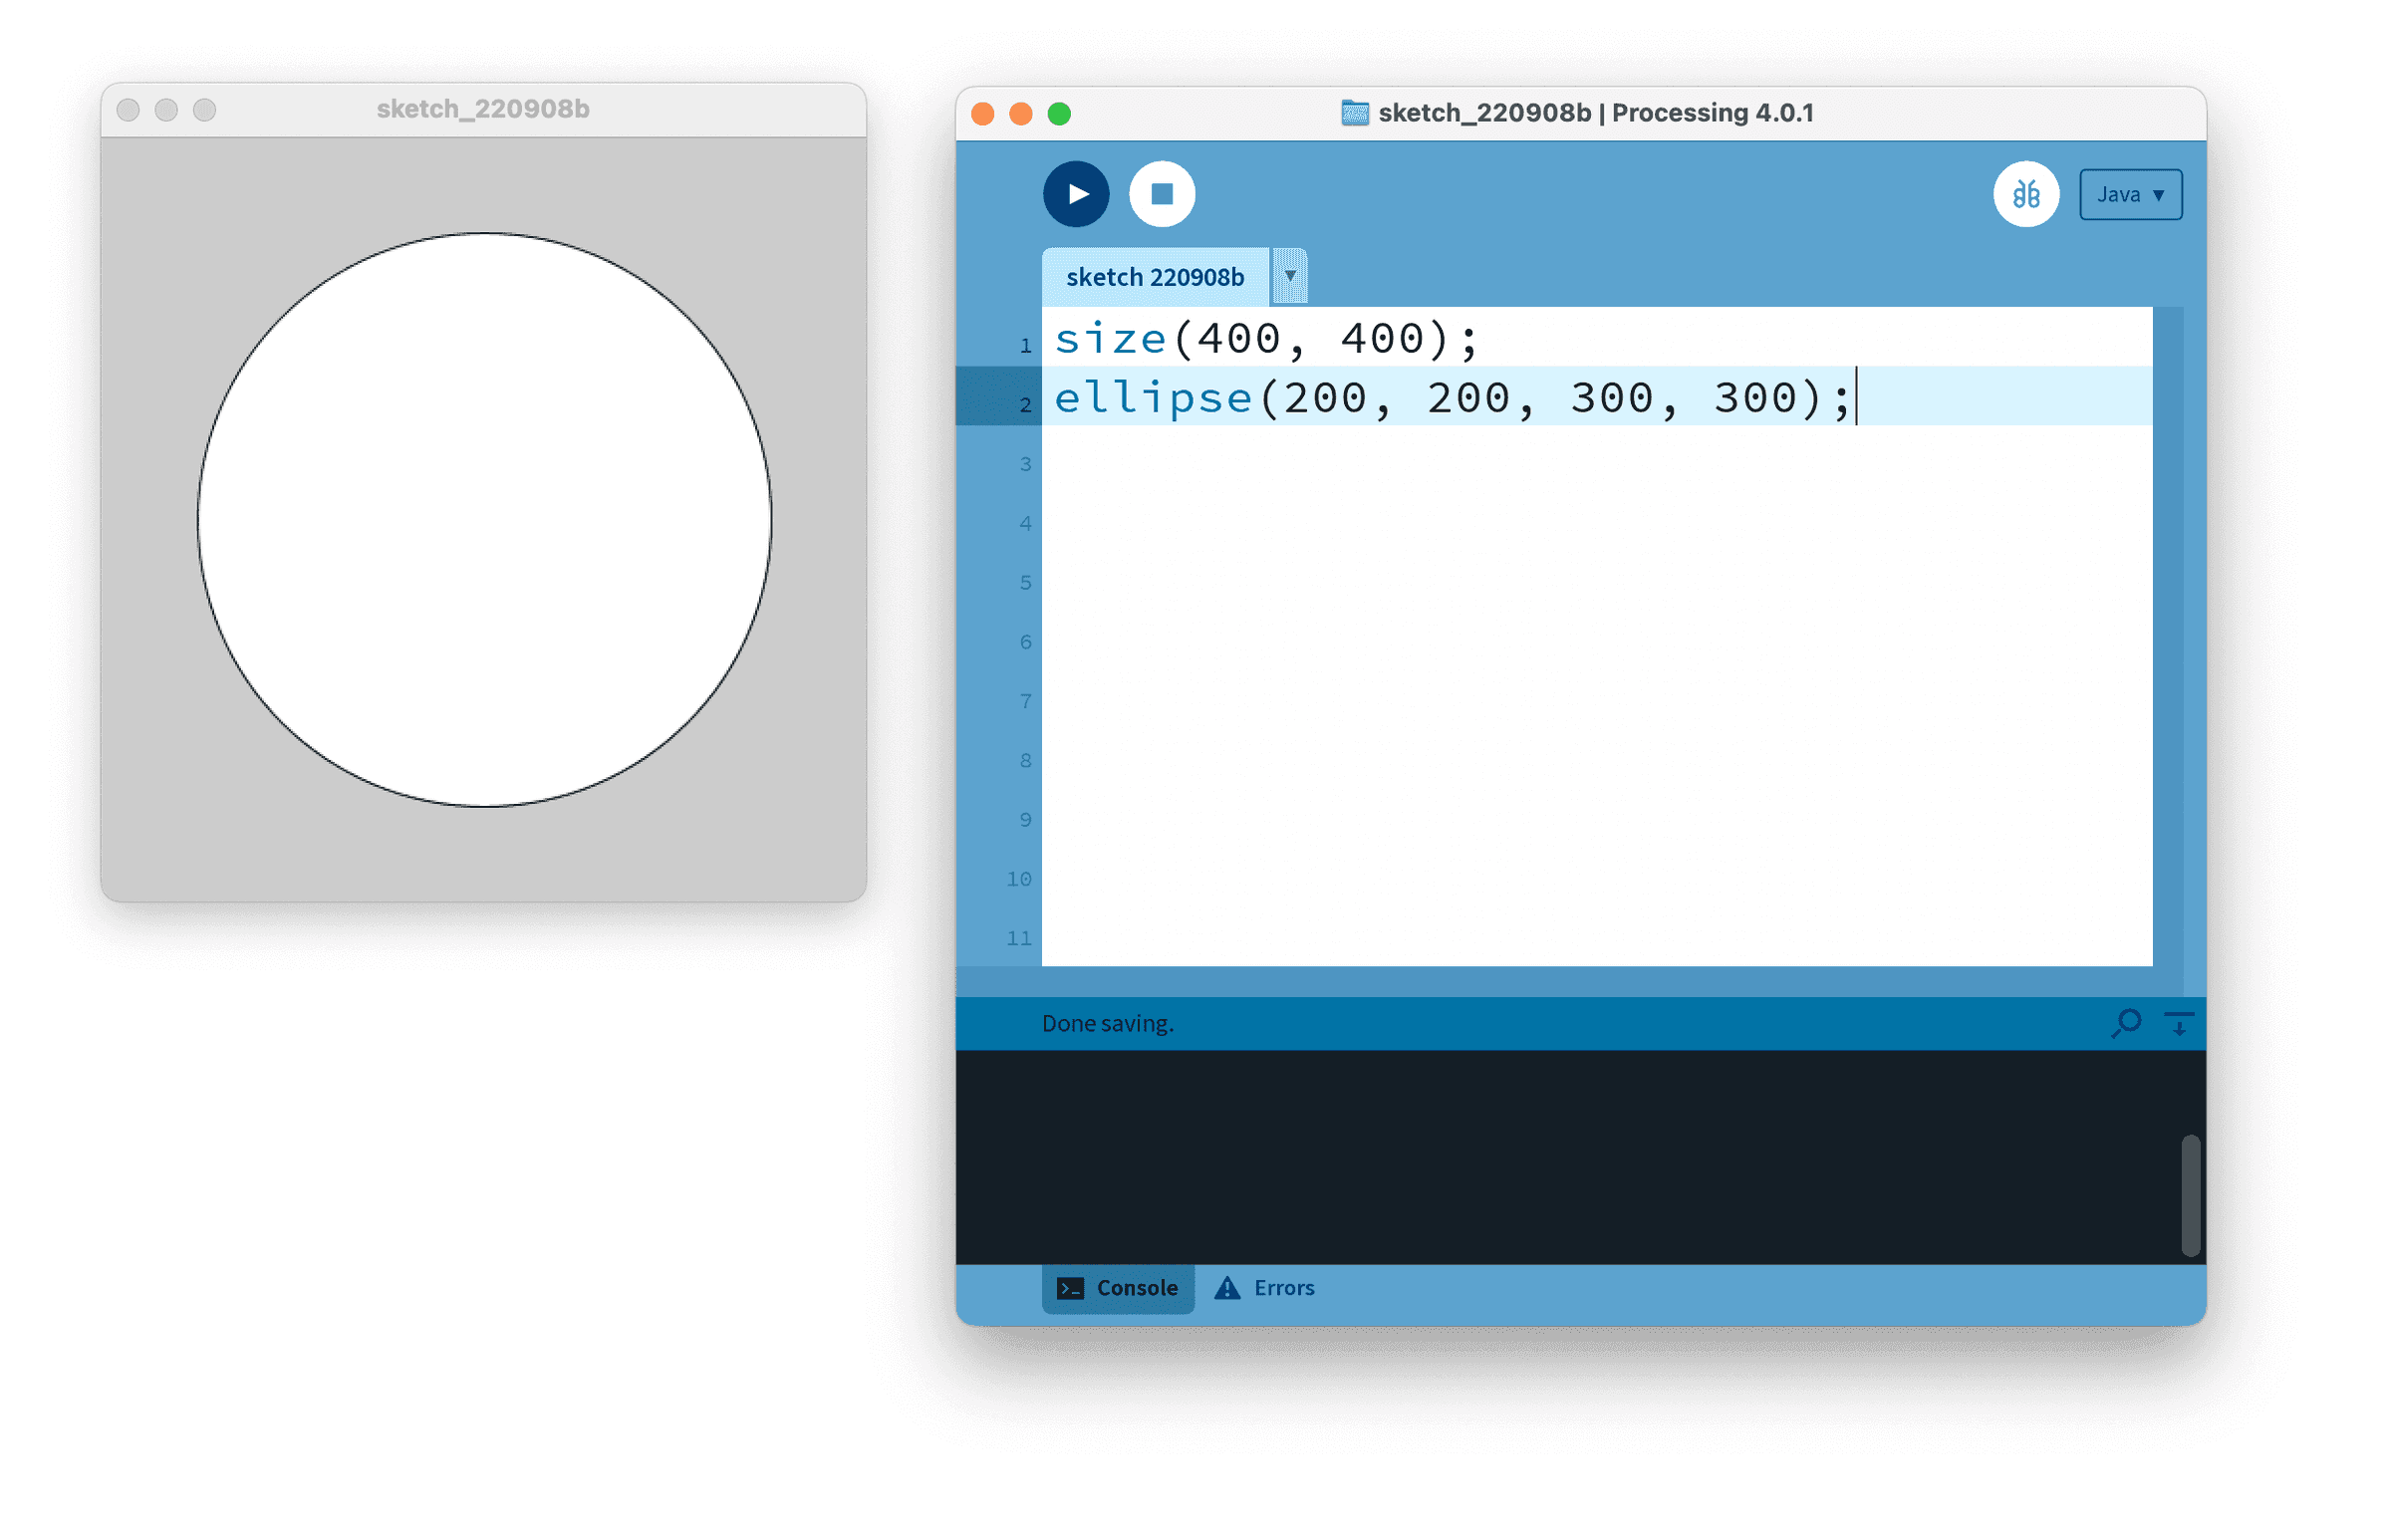
\includegraphics[width=1\textwidth]{images/processing_ide.png} 
    \caption{Processing IDE \parencite{reasProcessingIDE2015}}
    \label{fig:processing_ide_screenshot}
  \end{figure}
  

\subsection{The Legacy of Processing} % in Computational Design
%\subsection{The Enduring Legacy of Processing} % in Computational Design

Processing has marked its presence in the realm of digital design and creative coding with an enduring significance since its initial release on August 9, 2001 \parencite{processingfoundation20thAnniversaryProcessing2022}. This platform has not only persisted for over two decades but has also seen an expansion in its user base, indicating its continued relevance in a rapidly evolving field. Its role in shaping software literacy and education, especially for beginners, is well-documented, with its straightforward approach to coding and design principles that resonate with Maeda’s laws of simplicity \parencite{JohnMaedaLaws2020}.

The platform's design ethos, often aligned with principles such as "Low Threshold, High Ceiling, and Wide Walls," has facilitated a nurturing environment for learning and creation \parencite{resnickDesignPrinciplesTools}. The steady increase in the adoption of Processing, as indicated by user metrics that align with academic calendars, underscores its integration into educational structures \parencite{fryModernPrometheusHistory2018}. These metrics, alongside community surveys, suggest that Processing has transcended its educational utility, finding a place in professional workflows \parencite{2016CommunitySurvey}.

Processing's contribution to the field is further underlined by its influence on other significant projects, such as Arduino, which has roots in the same ethos and community \parencite{barraganUntoldHistoryArduino2016}. Its adaptability is evident through its evolution into variants like p5.js, Processing for Android, and Processing for Python, suggesting a responsive growth to the needs of its community, as visible on the Processing website.

In light of its historical context and the progressive adaptation to user needs, Processing stands as a distinguished example of enduring software in the creative coding community. It is this longevity and adaptability that prompt a closer examination of its design philosophy and community dynamics. As we witness the retirement of once-pivotal tools like Flash or Director, Processing's sustained relevance raises questions about the underlying factors contributing to its success \parencite{hortonDeathTechnicalSkill} \parencite{steveThoughtsFlashApple2010} \parencite{FutureAdobeContribute2019}.

However, despite its success and influence, a concerning aspect is the project's sustainability, considering the reliance on a small cadre of volunteer developers for the majority of the codebase \parencite{fryModernPrometheusHistory2018}. This situation poses significant questions about the long-term viability of open-source projects that are driven by community rather than commercial support.

\subsection{Research Questions}

In the preceding sections, we have contextualized Processing as a pivotal tool that has withstood the test of time, promulgating computational design and creative coding. Reflecting on Ben Fry's insightful perspective on Processing:

\begin{quote}
"The processing project is a community, a piece of software that you run, and a language. And that order is important." – Ben Fry \parencite[19:22]{artsatmit2017CASTSymposium2017}
\end{quote}

we understand the layered nature of the platform. This thesis seeks to unearth the dynamics that underpin the formation and perpetuation of a community around an open-source software such as Processing. The investigation pivots around a central research question:

\begin{quote}
"What were the foundational dynamics that not only instigated but also sustained the collaborative spirit of the Processing community? And how did these dynamics, entwined with the intrinsic motivations of open-source contributors, influence the evolution of Processing's software development over the years?"
\end{quote}

This question is aimed at dissecting the symbiotic relationship between community involvement and software innovation, probing into how the motivations of developers, particularly those contributing on a voluntary basis, shaped the trajectory of Processing's growth. The thesis will examine:

\begin{itemize}
\item The initial factors that attracted contributors to Processing and the elements that fostered their long-term engagement, as indicated by Fry's prioritization of the community.
\item The various forms of contributions made to the project, from coding to community support and education, reflecting the intertwined nature of the software and language.
\item The transformation of these community dynamics from the nascent stages of Processing to its present-day stature.
\item The underpinning reasons for continued voluntary participation in the project's development, despite the absence of direct financial incentives, aligning with Fry's understanding of the community's primacy.
\end{itemize}

The insights garnered from this exploration will augment our understanding of the sustainable models for the development of collaborative open-source software in the arts.

\subsection{Information sources}

% Research Design
Given the potential for memory bias due to the passage of time since the project's inception, this study employs a mixed-methods approach. While human memory can be fallible, introducing biases and even constructing false memories, quantitative analysis serves as a foundational component to mitigate these challenges. It allows for the identification of key contributors based on metrics such as commit frequency and significance, forum participation, and library contributions. These quantitative findings inform the selection of interviewees, acting as a preliminary filter to locate core contributors and library authors for qualitative interviews.

By purposefully integrating quantitative methodologies with qualitative ethnographic approaches, this research aspires to offer a nuanced understanding of both the structural and phenomenological aspects of the Processing community.

% Data Sources
The research draws upon multiple data sources to form a comprehensive picture of the Processing community and its development practices. These range from forum discussions at various phases of the project to commit histories and issue trackers. The parsing status indicates the extent to which each data source has been prepared for analysis. 


%\begin{table}[h]
    \raggedright
    \caption{Data sources}
    \label{table:data-sources}
    \begin{tabular}{l l l c}
        \toprule
        Name & Type & Status \\
        \midrule
        Processing alpha forum & Forum & Parsed \\
        Processing beta forum & Forum & Parsed  \\
        Processing 1.0 forum & Forum & Downloaded \\
        Processing 2.0 and 3.0 forum & Forum  & Not downloaded \\
        Current processing forum & Forum & Not downloaded\\
        Github project & Commit history & Parsed \\
        Processing Release Data & Release notes & Parsed \\
        Github Release Data & Release notes \& download statistics & Parsed \\
        Processing libraries\textsuperscript{*} & Software release information & Parsed \\

        \bottomrule
        \multicolumn{3}{l}{\footnotesize \textsuperscript{*}Note: The data set was reconstructed from the processing website archive and is not complete.}
    \end{tabular}
  \end{table}      


\begin{table}[h]
    \small
    %\adjustbox{max width=\textwidth}{
    \begin{adjustbox}{center}
    \begin{tabular}{l l l c}
        \toprule
        Name & Type & Status \\
        \midrule
        Processing alpha forum & Forum & Parsed \\
        Processing beta forum & Forum & Parsed  \\
        Processing 1.0 forum & Forum & Downloaded \\
        Processing 2.0 and 3.0 forum & Forum  & Not downloaded \\
        Current processing forum & Forum & Not downloaded\\
        Github project & Commit history & Parsed \\
        Processing Release Data & Release notes & Parsed \\
        Github Release Data & Release notes \& download statistics & Parsed \\
        Processing libraries\textsuperscript{*} & Software release information & Parsed \\
        Bugzilla & Software issue tracker & Not downloaded \\
        Github Issues & Software issue tracker & Not downloaded \\
        \bottomrule
        \multicolumn{3}{l}{\footnotesize \textsuperscript{*}Note: The data set was reconstructed from the processing website archive and is not complete.}
    \end{tabular}
    \end{adjustbox}
%} 
    \caption{Overview of Data Sources Used for Analyzing the Processing Community}
  \end{table}